%!TEX TS-program = xelatex
%!TEX encoding = UTF-8 Unicode

\documentclass[12pt]{article}
\usepackage{geometry}                % See geometry.pdf to learn the layout options. There are lots.
\geometry{a4paper,top=2cm}
\usepackage[parfill]{parskip}    % Activate to begin paragraphs with an empty line rather than an indent
\usepackage{graphicx}
\usepackage{amsmath}
\usepackage{amssymb}
\usepackage{mathtools}
\usepackage{physics}
\newcommand{\be}{\begin{equation}}
\newcommand{\ee}{\end{equation}}
\usepackage[thicklines]{cancel}
\usepackage[colorlinks=true,citecolor=blue,linkcolor=blue,urlcolor=blue]{hyperref}
\usepackage{booktabs}
\usepackage{csquotes}
\usepackage{qcircuit}
\usepackage{circledsteps}
\usepackage{nicefrac}
\usepackage{fontspec,xltxtra,xunicode}
\usepackage{xcolor}
\usepackage{simplewick}
\defaultfontfeatures{Mapping=tex-text}

\newcommand{\polv}{\ensuremath{\updownarrow}}
\newcommand{\polh}{\ensuremath{\leftrightarrow}}
\newcommand{\poldr}{\rotatebox[origin=c]{45}{\ensuremath{\leftrightarrow}}}
\newcommand{\poldl}{\rotatebox[origin=c]{-45}{\ensuremath{\leftrightarrow}}}
\newcommand{\bigzero}{\mbox{\normalfont\Large\bfseries 0}}
\newcommand{\vecrp}{\ensuremath{\vec{r}^{\,\prime}}}
\newcommand{\vecnr}{\ensuremath{\vec{\nabla}_{\!r}}}

\usepackage{fontspec,xltxtra,xunicode}
\defaultfontfeatures{Mapping=tex-text}

\title{Advanced Quantum Mechanics\\Class 08--09}
%\author{The Author}
\date{September 01, 2022}                                           % Activate to display a given date or no date

\setcounter{section}{5}
\setcounter{subsection}{7}
\setcounter{equation}{81}

\begin{document}
\maketitle

%%% 5, aula 08

\subsection{EPR argument \& Bell inequalities}

EPR: Einstein--Podolsky--Rosen.

\begin{enumerate}
\item Suppose a particle of spin 0 decays into other two
each with spin \(1 / 2\).
%
\item Suppose two experimentalists, A (Alice) and \(B\) (Bob) ,
for apart from each other, measure the spin projection
on certain directions: A in direction \(\hat{a}\) and \(B\) in \(\hat{b}\),
conventionally on a plane perpendicular to the
propagation of the two particles).
%
\begin{center}
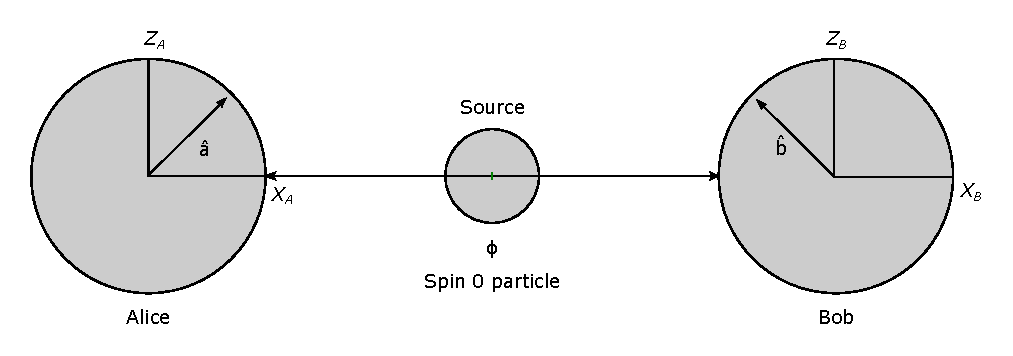
\includegraphics[width=\textwidth]{Figures/EPR_illustration.pdf}
\end{center}
\item  Suppose, first \(\hat{a}=b=\hat{z}\). Results: if \(A\) finds
\(+\hbar / 2, B\) finds \(-\hbar / 2\); if \(A\) finds \(-\hbar / 2, B\) finds \(+\hbar / 2\)
$\rightarrow$
that is: the correlation of the measurements
is always \(-\hbar^{2} / 4\).
\end{enumerate}
Interpretation: the state of the two spins due to
%%% 6, aula 08 OK
angular momentum conservation, is
\be
\ket{\Phi} = \frac{1}{\sqrt{2}}
\left(\ket{-+} - \ket{+-}\right)
\ee
We observe that this state is an eigenstate of
$S_{z}^{a} \otimes S_{z}^{b}$:
\be
S_{z}^{a} \otimes S_{z}^{b}\ket{\Phi} = \frac{\hbar^2}{4} \ket{\Phi}
\ee
therefore correlation  of the measurements of $A$ and $B$
\emph{must} give $\frac{\hbar^2}{4}$.

Le Bellac's two travellers \(a\) and \(b\) are given a
suitcase each, one containing a red ball and
the other a green ball. At customs checking points,
at different air ports, customs officers \(A\) and \(B\)
open the suitcases: if A finds red, B finds green;
$\Rightarrow$
Correlation between the suitcases were
introduced at the time of departure
--- they are revealed when measurements
are made.

\begin{enumerate}
\setcounter{enumi}{2}
\item Suppose now \(\vec{a}=\hat{b}=\hat{x}\). Nothing changes with
respect to outcomes of measurements, since $\ket{\Phi}$ is
rotationally invariant (as seen before), \((\Phi)\) is an
eigenstate of \(\hat{S}_{x}^{(a)} \otimes \hat{S}_{x}^{(b)}\) with eigenvalue \(-\hbar^{2} / 4\):
%%% 7, aula 08 OK
rotationally invariant (as seen before), $\ket{\Phi}$ is an
eigenstate of $S_{x}^{a} \otimes S_{x}^{b}$ with eigenvalue $-\hbar^2/4$:
\[
S_{x}^{a} \otimes S_{x}^{b}\ket{\Phi} = -\frac{\hbar^2}{4} \ket{\Phi}
\]

\item EPR argument to explain these results:
``realism'' + ``locality principle''
\begin{itemize}
\item\emph{Realism:} microscopic systems possess intrinsic
properties which most have a counterpart
in the physical theory.
``If the value of a physical property can be predicted
with certainty without disturbing the system in any
way there is an element of reality associated with
this property'' -- \textit{e.g.} $\hat{S}_x$ and $\hat{S}_y$ have simultaneously well defined values.
\item\emph{Locality principle:} if \(A\) and \(B\) make their measurements
in local regions of spacetime which cannot be
causally connected, then it is not possible that
an experimental parameter chosen by \(A, e . g\). The
orientation of her Stern-Gerlach apparatus, can affect
the properties of particle b.
\end{itemize}
\end{enumerate}

Our examples in 2. and 3.: a measurement of
\(S_{z}^{(a)}\) permits to predict \(S_{z}^{(b)}\) with certainty
without disturbing b. Same with for \(\hat{S}_{x}\).

%%% 8, aula 08 OK

\emph{According to EPR} ``local realism'': result of \(A\)
measurement serves only to reveal a piece of
information that was already stored in the local
region of spacetime associated with particle b.

Fine, in the examples correlations were built in, \emph{BUT}
``local realism'' would also imply that a theory
respecting this principle would contain simultaneous 
complete information on \(\hat{S}_{x}^{(b)}\) and \(\hat{S}_{z}^{(b)}\) and be
able to predict with certainty when measuring these
properties $\to$ EPR agree that QM gives result
that are \emph{statistically} correct, but
QM is not sufficient for describing
the ``physical reality'' of an individual
pair.

How to decide? \emph{Experiment}.

Devise measurements such that one can
clearly distinguish predictions bared on QM
and ``local realism'' $\to$ Bell inequalities.

%%% 1, aula 09

Local realism: even if an experiment cannot
measure (due to e.g. a technical problem)
simultaneously \(S_{x}^{(b)}\) and \(S_{y}^{b)}\), these two
quantities \emph{do have} a simultaneous physical
reality in the local region of spacetime
attached to particle b $\rightarrow$
by symmetry, same is true
for \(S_{x}^{(a)}\) and \(S_{y}^{(a)}\) of particle a.

\emph{Bell inequalities}\,$\rightarrow$\,fix the maximum possible
correlations given this hypothesis.
\[
\text{\emph{Notation:} }
\left\{
\begin{aligned}
\hat{a}, \hat{a}^\prime:&\text{ axes used by } A\\
\hat{b}, \hat{b}^\prime:&\text{ axes used by } B
\end{aligned}
\right.
\]

To avoid \(\hbar / 2\) factors, instead of \(\vec{s}\) use \(\vec{\sigma}\)
\(A(\hat{a})\) : result of measurement \(\vec{\sigma}\) in direction \(\hat{a}\) by \(A\)
same for \(B(\vec{b})\) )
\be
\begin{aligned}
\vec{\sigma}^{(a)}_{\hat{a}}&=
\vec{\sigma}^{(a)} \cdot \hat{a} \rightarrow \vec{\sigma} \cdot \hat{a}\\
\vec{\sigma}^{(b)}_{\hat{b}}&=
\vec{\sigma}^{(b)} \cdot \hat{b} \rightarrow \vec{\sigma} \cdot \hat{b}
\end{aligned}
\ee
Possible results of the measurement are $\pm1$:
\be
A(\hat{a})=\varepsilon_{a}=\pm 1\,,\,B(\hat{b})=\varepsilon_{b}=\pm 1
\ee
same for any other $\hat{a}^\prime$, $\hat{b}^\prime$.
%%% 2, aula 09 OK
$P_{\varepsilon_a \varepsilon_b}$: joint probability for $A$ find $\varepsilon_a$ and $B$ find $\varepsilon_b$.
\be
\begin{aligned} 
E(\hat{a}, \hat{b}) 
&=\sum_{\varepsilon_{a}, \varepsilon_{b}} \varepsilon_{a} \varepsilon_{b} P_{\varepsilon_{a} \varepsilon_{b}} \\ 
&=\left(p_{++}+p_{--}\right)-\left(p_{+-}+p_{-+}\right)
\end{aligned}
\label{eq:g86}
\ee
and experimentally, this is:
\be
[E(\hat{a}, \hat{b})]_{\text{exp}}=\lim _{N \rightarrow \infty} \frac{1}{N} \sum_{n=1}^{N} A_{n}(\hat{a}) B_{n}(\hat{b})
\ee
that is independent of theory, it is an experiment quantity.

Before going to calculate the predictions of QM
for different axes, let us consider the following
combination of correlation measurements:
\be
\begin{aligned} 
X_{n} 
&=A_{n}(\hat{a}) B_{n}(\hat{b})+A_{n}(\hat{a}) B_{n}(\hat{b}^{\prime})+A_{n}(\hat{a}^{\prime}) B_{n}(\hat{b}^{\prime})\underbrace{\pmb{\boldsymbol{-}}}%
_{\mathrlap{\text{Bell's insight}}}
A_{n}(\hat{a}^{\prime})B_{n}(\hat{b})\\ 
&=A_{n}(\hat{a})\left[B_{n}(\hat{b})+B_{n}(\hat{b}^{\prime})\right]+A_{n}(\hat{a}^{\prime})\left[B_{n}(\hat{b}^{\prime})-B_{n}(\hat{b})\right]
\end{aligned}
\label{eq:g88}
\ee
\emph{Note that:} only one of the four combinations in
\eqref{eq:g88} can be measured \emph{on a pair n},
%%% 3, aula 09
\emph{BUT} the \emph{possible} results for the three other
experiments (values of course unknown) is well
defined in QM \emph{and} ``local realism''.

\emph{In QM:} 
$A(\hat{a})B(\hat{b}) \to E(\hat{a},\hat{b})$,
$A(\hat{a})B(\hat{b}^\prime) \to E(\hat{a},\hat{b}^\prime)$, \ldots
all given in terms of probabilities $p_{++}$, $p_{+-}$, \ldots $\to$ Eq.\eqref{eq:g86}

\emph{``Local realism'':}
$A_{n}(\hat{a})=\pm 1$, $B_{n}(\hat{b})=\pm 1$, $A_{n}(\hat{a}^\prime)=\pm 1$, \ldots.
What is the value of $X_n$?
\be
\begin{gathered}
\text{For } B_n(\hat{b}) =  B_n(\hat{b}^\prime) \to 
X_n = 2 A_{n}(\hat{a}) B_n(\hat{b}) = \pm 2\\
\text{For } B_n(\hat{b}) =  -B_n(\hat{b}^\prime) \to 
X_n = 2 A_{n}(\hat{a}^\prime) B_n(\hat{b}) = \pm 2\\
\end{gathered}
\ee
average over a large number of experiments, leads to an absolute value
\be
\begin{aligned}
|\langle X\rangle|_{\text{EPR}}
&=\left|\lim _{N \rightarrow \infty} \frac{1}{N} \sum_{n=1}^{N} X_{n}\right|\\
&=|\lim _{N \rightarrow \infty} \frac{1}{N} 
\underbrace{(\pm 2 \pm 2 \pm 2 \cdots \pm 2)}_{N}| \leqslant 2
\end{aligned}
\ee
(in case of equality: all $+2$ or $-2$). And finally:
\be
|\langle X\rangle|_{\text{EPR}} \leqslant 2
\ee
and example of a Bell inequality.

%%% 4, aula 09 OK

EPR result was derived under the hypothesis
that particle $a$ possesses properties 
\(A_{n}(\hat{a})\) and
\(A_{n}(\hat{a}^{\prime})\) simultaneously, and $b$ possesses
\(B_{n}(\hat{b})\) and 
\(B_{n}(\hat{b}^{\prime})\)
and \(A_{n}(\hat{a})\) cannot depend on the orientation
of \(\hat{b}\) or \(\hat{b}^{\prime}\) chosen by Bob.

\emph{Quantum mechanics}: First, let us calculate \(E(\hat{a}, \hat{b})\)
for generic axes $\hat{a}$ and $\hat{b}$: $\hat{a}$ can always be chosen
$\hat{a}=\hat{z}$. For a general $\hat{b}: \hat{b}$ angle $\theta$ with $\hat{z}$.
\be
\text { Eigenstates of } \vec{\sigma} \cdot \hat{a}=\sigma_{z}: \ket{+},\ket{-}
\ee
\be
\text { Eigenstates of } \vec{\sigma} \cdot \hat{b}\left\{
\begin{array}{l}
\ket{+, \hat{b}}= \cos \theta / 2|+\rangle+\sin \theta / 2|-\rangle \\ 
\ket{-, \hat{b}}=-\sin \theta / 2|+\rangle+\cos \theta / 2|-\rangle
\end{array}\right.
\ee

On decay, state of the two particles is, in the basis
\(\{|+\rangle,|-\rangle\},|\Phi\rangle=\frac{1}{\sqrt{2}}[|+-\rangle-|-+\rangle]\)

\(p_{++}\): probability finding 
\(\vec{\sigma} \cdot \hat{a}\) in \(\ket{+}\) and 
\(\vec{\sigma} \cdot \hat{b}\) in \(\ket{+}\)

\be
\begin{aligned} 
p_{++} 
&=|\langle+|\otimes\langle +, \hat{b} \mid \Phi\rangle|^{2}\\ 
&=\left|\sin \theta / 2 \frac{1}{\sqrt{2}}\langle+-\mid+-\rangle\right|^{2}=
\frac{1}{2} \sin ^{2} \theta / 2 
\end{aligned}
\ee
Likewise:
\be
p_{+-} = \left|\bra{+}\otimes\bra*{-,\hat{b}}\ket*{\Phi}\right|^2 = 1/2\cos^2\theta/2
\ee
%%% 5, aula 09 (falta o plot dos eixos)
\be
p_{-+} = \left|\bra{-}\otimes\bra*{+,\hat{b}}\ket*{\Phi}\right|^2 = 1/2\cos^2\theta/2
\ee
\be
p_{--} = \left|\bra{-}\otimes\bra*{-,\hat{b}}\ket*{\Phi}\right|^2 = 1/2\sin^2\theta/2
\ee

\be
\begin{aligned} 
E\left(\hat{a}, \hat{b}\right) 
&=\left(p_{++}+p_{--}\right)-\left(p_{+-}+p_{-+}\right) \\
&=\sin ^{2} \theta / 2-\cos ^{2} \theta / 2=-\cos \theta \\ 
&=-\hat{a} \cdot \hat{b} 
\end{aligned}
\ee

Now, a specific choice of axes:

\begin{minipage}{0.45\textwidth}
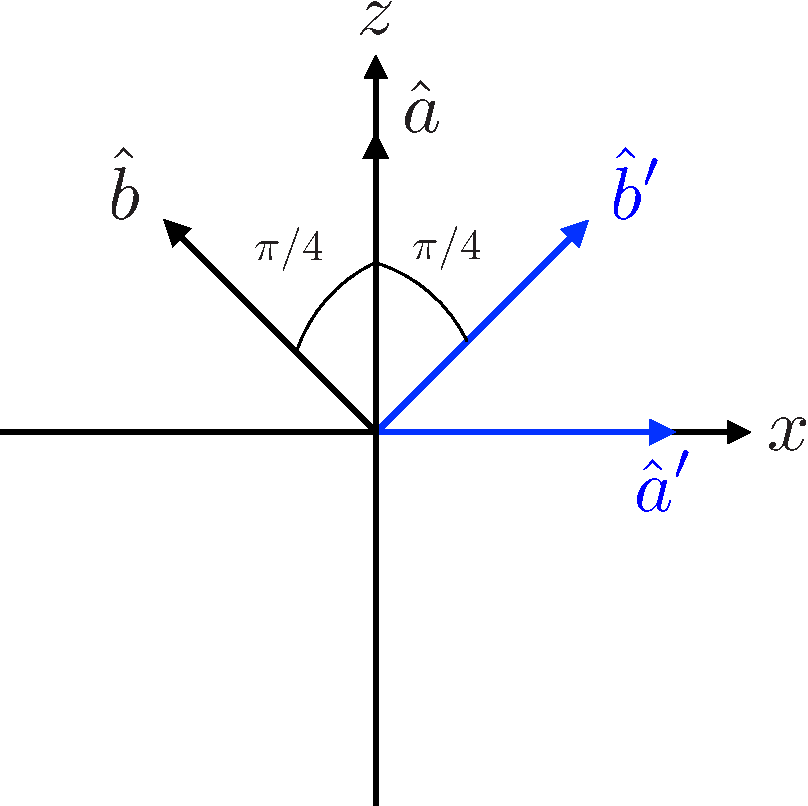
\includegraphics[width=\textwidth]{Figures/Bell-axes-crop.pdf}
\end{minipage}%
\hfill%
\begin{minipage}{0.45\textwidth}
\be
\begin{aligned}
&\hat{a}=\hat{z},\,         &\hat{b}=-\pi / 4 \\ 
&\hat{a}^{\prime}=\pi / 2,\,&\hat{b}^{\prime}=\pi / 4
\end{aligned}
\label{eq:g99}
\ee
Using rotational invariance of $\ket{\Phi}$:
\end{minipage}

\be
\begin{aligned}
E(\hat{a}, \hat{b})=-\frac{1}{\sqrt{2}},\quad 
& E\left(\hat{a}, \hat{b}^{\prime}\right)=-\frac{1}{\sqrt{2}} \\ 
E(\hat{a}^{\prime}, \hat{b})=+\frac{1}{\sqrt{2}},\quad 
& E\left(\hat{a}^{\prime}, \hat{b}^{\prime}\right)=-\frac{1}{\sqrt{2}}
\end{aligned}
\ee
Therefore, \emph{for this choice of axes}, $\ev{X}$ is given by
\be
\begin{gathered}
E(\hat{a}, \hat{b}) + E(\hat{a}, \hat{b}^{\prime}) +
E(\hat{a}^{\prime}, \hat{b}^{\prime}) -
E(\hat{a}^{\prime}, \hat{b})\\
= -\frac{1}{\sqrt{2}} -\frac{1}{\sqrt{2}} -\frac{1}{\sqrt{2}} -\frac{1}{\sqrt{2}} 
= -\frac{4}{\sqrt{2}} = -2\sqrt{2}
\end{gathered}
\ee
and the modulus of $\ev{X}$ is
%%% 6, aula 09 OK
\be
|\ev{X}| = 2\sqrt{2}\to\text{ for choice of axis Eq.\eqref{eq:g99}}
\ee
This choice of axes maximizes $|\ev{X}|$ (try showing this). Therefore:
\be
|\ev{x}|^{\text{QM}}_{\max} = 2\sqrt{2}
\ee
\be
\text{QM violates EPR: } |\ev{X}|^{\text{EPR}}_{\max} = 2
\ee
Quantum correlations are stronger than
those implied by ``local realism''.

\emph{Contradiction} with EPR comes from the fact that
in QM one cannot attribute well-defined values
to the four 
\(A_{n}\left(\hat{a}\right), 
  A_{n}\left(\hat{a}^{\prime}\right), 
  B_{n}(\hat{b})\) and
\(B_{n}(\hat{b}^{\prime})\) for
a single pair of spin 1/2 particles $\to$
they correspond to eigenvalues of
operators that do not commute
with each other.





















\end{document}